\documentclass[11pt]{article}
\usepackage{amsmath, amssymb, physics, mathtools, bm}
\usepackage{tikz, pgfplots}
\usetikzlibrary{calc, positioning, decorations.markings}
\pgfplotsset{compat=1.18}
\usepackage[margin=2.3cm]{geometry}
\usepackage{siunitx, booktabs, hyperref}

\newcommand{\D}{\mathrm{D}}
\newcommand{\de}{\mathrm{d}}
\newcommand{\pd}[2]{\frac{\partial #1}{\partial #2}}
\newcommand{\pdd}[2]{\frac{\partial^{2} #1}{\partial #2^{2}}}
\newcommand{\Lap}{\nabla^{2}}
\newcommand{\fourv}[1]{\mathsf{#1}}
\DeclareMathOperator{\diag}{diag}

\title{B2 Symmetry and Relativity, 2021 --- Model Solutions}
\author{}
\date{}

\begin{document}
\maketitle

%==================================================================
\section*{Question 1 --- Charges in a uniform electric field}

\textbf{Problem.} Electron at $x=0$, positron at $x=+d$, both at rest in $S$. At $t=0$ a constant field $\vb E$ is switched on. (a) world lines for $\vb E=E\hat{\vb x}$; (b) motion in $S'$ moving at $v\hat{\vb x}$ and momentum status; (c) for $\vb E=-E\hat{\vb x}$ with $d=\SI{20}{cm}$, $E=\SI{50}{kV/cm}$, find KE at collision, $N_{\min}$, photon $\lambda$; (d) minimum $d$ to produce $W^+W^-$, and linear vs.\ circular colliders.

\subsection*{(a)}

Forces: electron feels $-eE\hat{\vb x}$, positron $+eE\hat{\vb x}$. They accelerate apart.

Equation of motion for positron, $\de p/\de t = qE$:
\[ p(t) = qEt. \]
Total energy from $E_{\rm tot}^2=p^2c^2+m^2c^4$:
\[ E_{\rm tot}(t) = \sqrt{m_e^2 c^4 + q^2 E^2 t^2 c^2}. \]
Velocity from $v = p c^2/E_{\rm tot}$:
\[ v(t) = \frac{qEt\,c^2}{\sqrt{m_e^2 c^4 + q^2 E^2 t^2 c^2}}. \]
Integrate with $x(0)=x_0$:
\[ x(t) - x_0 = \int_0^t \frac{qEt'\,c^2\,\de t'}{\sqrt{m_e^2 c^4 + q^2 E^2 t'^2 c^2}}. \]
Substitute $a_0 = eE/m_e$:
\begin{equation}
x(t) = x_0 + \frac{c^2}{a_0}\!\left[\sqrt{1+(a_0 t/c)^2}-1\right],\quad a_0=eE/m_e.
\label{eq:hyperbolic}
\end{equation}
Each world line is a hyperbola: vertical tangent at $t=0$, asymptote at slope $\pm 1/c$. Mirror-symmetric about $x=d/2$.

\begin{center}
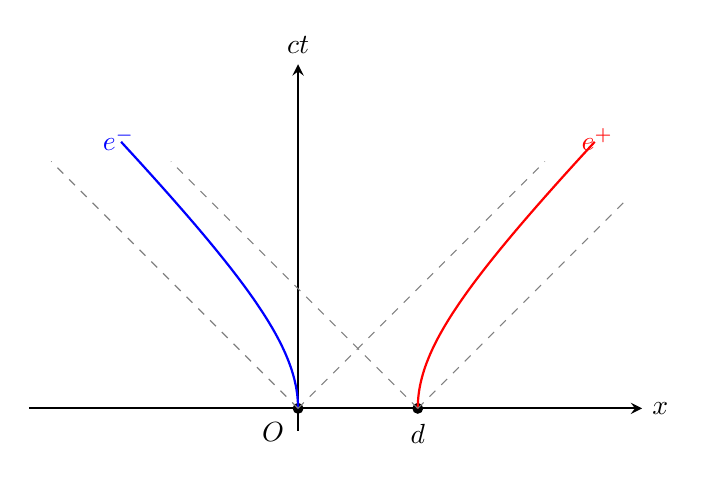
\begin{tikzpicture}[>=stealth, scale=0.95]
  \draw[->, thick] (-3.6,0) -- (4.6,0) node[right] {$x$};
  \draw[->, thick] (0,-0.3) -- (0,4.6) node[above] {$ct$};
  \node[circle,fill,inner sep=1.4pt,label=below left:{$O$}] at (0,0) {};
  \node[circle,fill,inner sep=1.4pt,label=below:{$d$}] at (1.6,0) {};
  % electron hyperbola (left)
  \draw[thick,blue,domain=0:1.6,smooth,variable=\u]
       plot ({-1.5*(cosh(\u)-1)}, {1.5*sinh(\u)});
  \node[blue] at (-2.4,3.6) {$e^-$};
  % positron hyperbola (right)
  \draw[thick,red,domain=0:1.6,smooth,variable=\u]
       plot ({1.6+1.5*(cosh(\u)-1)}, {1.5*sinh(\u)});
  \node[red] at (4.0,3.6) {$e^+$};
  % light cones from each start
  \draw[gray,dashed] (0,0) -- (-3.3,3.3);
  \draw[gray,dashed] (0,0) -- (3.3,3.3);
  \draw[gray,dashed] (1.6,0) -- (-1.7,3.3);
  \draw[gray,dashed] (1.6,0) -- (4.4,2.8);
\end{tikzpicture}
\end{center}

\boxed{\;\text{Mirror hyperbolae about }x=d/2,\; a_0=eE/m_e.\;}

\subsection*{(b)}

In $S'$ the surfaces $t'=\,$const tilt: events ``field on at electron'' (origin) and ``field on at positron'' $(d,0)$ are not simultaneous in $S'$. Apply Lorentz transformation $t' = \gamma(t - vx/c^2)$:
\[ t'_{\rm e^-} = 0,\qquad t'_{\rm e^+} = -\gamma v d/c^2. \]
Time gap:
\[ \Delta t' = t'_{\rm e^+} - t'_{\rm e^-} = -\gamma v d/c^2. \]
For $v>0$ the positron's switch-on lies at \emph{earlier} $t'$. So in $S'$ the positron accelerates first while the electron remains at rest.

Trajectories remain hyperbolic (boost along $\hat{\vb x}$ maps hyperbolic motion to hyperbolic motion) but no longer mirror-symmetric.

Total 3-momentum in $S$: forces equal and opposite:
\[ \dot{\vb P}_{\rm tot} = -eE\hat{\vb x} + eE\hat{\vb x} = 0. \]
Hence $\vb P_{\rm tot}$ conserved in $S$.

In $S'$: $E'_x=E_x$, but during the simultaneity-mismatch interval only one particle accelerates:
\[ \dv{\vb P'_{\rm tot}}{t'} = +eE\hat{\vb x}'\quad\text{(transient, positron only)}. \]
Hence $\vb P'_{\rm tot}$ \emph{not} conserved during the transient: external (field) source is non-simultaneous in $S'$, so the system is open.

\textbf{4-vector status.} Each $\fourv P_i$ is a 4-vector. The sum $\sum_i \fourv P_i(t)$ depends on the spacelike slice ($t=$const in $S$ vs.\ $t'=$const in $S'$). For an isolated system the slice-dependence drops out and the total is a 4-vector; for our open system (field on, particles still in field), the slice matters and $\fourv P_{\rm tot}$ is not a 4-vector.

\boxed{\;\vb P_{\rm tot}\text{ conserved in }S;\text{ not in }S'\text{ during transient};\;\fourv P_{\rm tot}\text{ a 4-vector only for closed system.}\;}

\subsection*{(c)}

Reverse field: electron pushed $+\hat{\vb x}$, positron $-\hat{\vb x}$. They meet at $x=d/2$ by symmetry. Each crosses distance $d/2$.

Work--energy theorem with force $eE$ over distance $d/2$:
\[ T = eE\,\frac{d}{2}. \]
Convert field: $E = \SI{50}{kV/cm} = \SI{5e6}{V/m}$:
\[ T = e\times\SI{5e6}{V/m}\times\SI{0.10}{m}. \]
Evaluate:
\[ T = \SI{5e5}{eV}. \]
Hence
\boxed{\;T = \SI{0.500}{MeV}\text{ per particle.}\;}

Total energy in lab equals ZMF energy by symmetry:
\[ E_{\rm tot} = 2(m_ec^2 + T). \]
Substitute:
\[ E_{\rm tot} = 2(\SI{0.511}{MeV}+\SI{0.500}{MeV}). \]
Evaluate:
\[ E_{\rm tot} = \SI{2.022}{MeV}. \]

\textbf{Photon number.} ZMF total $\bm p=0$. Single photon has $|\bm p_\gamma|=E_\gamma/c\neq 0$: forbidden. Two photons back-to-back conserve both energy and momentum:
\boxed{\;N_{\min}=2.\;}

\textbf{Wavelength.} Each photon carries half the total energy:
\[ E_\gamma = E_{\rm tot}/2 = \SI{1.011}{MeV}. \]
Apply $\lambda = hc/E_\gamma$ with $hc=\SI{1240}{eV.nm}$:
\[ \lambda = \frac{\SI{1240}{eV.nm}}{\SI{1.011e6}{eV}}. \]
Evaluate:
\boxed{\;\lambda \approx \SI{1.23}{pm}.\;}

\subsection*{(d)}

Threshold for $e^+e^-\to W^+W^-$ requires $E_{\rm tot}\ge 2m_W c^2$:
\[ 2(m_ec^2 + T_{\min}) = 2 m_W c^2. \]
Neglect $m_e c^2 \ll m_W c^2$:
\[ T_{\min} = m_W c^2 - m_e c^2 \approx m_W c^2 = \SI{80.379}{GeV}. \]
Use $T_{\min}=eE\,d_{\min}/2$ from (c):
\[ d_{\min} = \frac{2 T_{\min}}{eE} = \frac{2 m_W c^2}{eE}. \]
Substitute $eE=\SI{5e6}{eV/m}$:
\[ d_{\min} = \frac{2\times\SI{80.379e9}{eV}}{\SI{5e6}{eV/m}}. \]
Evaluate:
\boxed{\;d_{\min}\approx \SI{32}{km}.\;}

\textbf{Linear vs.\ circular.} Synchrotron loss per turn $\propto \gamma^4/r$; for electrons at TeV scale $\gamma\sim 10^6$, prohibitive. Linear: no centripetal $a$, no synchrotron loss; ideal for $e^\pm$ at high energy. But single-pass: low luminosity. Circular: ideal for protons ($\gamma_p/\gamma_e = m_e/m_p$), continuous bunch reuse, high luminosity (LHC).

%==================================================================
\section*{Question 2 --- Liénard--Wiechert and synchrotron radiation}

\textbf{Problem.} (a) Derive $A^\mu$ for an arbitrarily moving charge; explain radiative vs.\ non-radiative. (b) Synchrotron $r=\SI{500}{m}$, $B=\SI{0.02}{T}$: find $\gamma$, $E$, energy loss per turn (Larmor). (c) Detector at $+\hat{\vb x}$: show pulses, estimate duration.

\subsection*{(a)}

Define source 4-velocity at retarded proper time:
\[ U^\mu = \de X^\mu/\de\tau,\qquad U\cdot U = -c^2. \]
Define retarded null separation from source to observer:
\[ R^\mu = X^\mu_{\rm obs} - X^\mu(\tau_{\rm ret}),\quad R\cdot R = 0,\quad R^0 > 0. \]
Ansatz, manifestly a 4-vector:
\begin{equation}
A^\mu = \frac{q}{4\pi\epsilon_0}\,\frac{U^\mu/c}{-R_\nu U^\nu}.
\label{eq:LW}
\end{equation}
Verify in instantaneous rest frame at retarded event: $U^\mu = (c,\bm 0)$, $R^\mu=(r,\bm r)$ with $r=|\bm r|$.

Lower index in metric $\diag(-,+,+,+)$:
\[ R_0 = -r,\qquad R_i = r^i. \]
Contract with $U^\mu$:
\[ R_\nu U^\nu = (-r)(c) + 0 = -rc. \]
Hence:
\[ -R_\nu U^\nu = rc. \]
Substitute into ansatz with $U^\mu/c = (1,\bm 0)$:
\[ A^\mu_{\rm rest} = \frac{q}{4\pi\epsilon_0}\,\frac{(1,\bm 0)}{rc} = \left(\frac{1}{c}\frac{q}{4\pi\epsilon_0 r},\;\bm 0\right). \]
Recognise static Coulomb $A^0 = \phi/c$. Both sides are 4-vectors; agreement in one frame $\Rightarrow$ all frames.

General frame: $U^\mu=\gamma(c,\bm v)$ and $R^\mu = (r,\bm r)$ with $r=|\bm r|$. Contract:
\[ -R_\nu U^\nu = -(-r)(\gamma c) - \bm r\cdot\gamma\bm v = \gamma c r - \gamma\, r\,\hat{\bm r}\cdot\bm v. \]
Factor:
\[ -R_\nu U^\nu = \gamma c r\,\kappa,\qquad \kappa \equiv 1-\hat{\bm r}\cdot\bm v/c. \]
Read off scalar and vector potentials:
\[ \phi = \frac{1}{4\pi\epsilon_0}\frac{q}{r\kappa}\bigg|_{\rm ret},\qquad \bm A = \frac{\mu_0}{4\pi}\frac{q\bm v}{r\kappa}\bigg|_{\rm ret}. \]

\textbf{Field structure.} $\bm E = -\nabla\phi - \partial_t\bm A$; chain rule through $t_{\rm ret}$ yields
\[ \bm E = \frac{q}{4\pi\epsilon_0}\!\left[\underbrace{\frac{(\hat{\bm r}-\bm v/c)(1-v^2/c^2)}{\kappa^3 r^2}}_{\text{velocity, }\propto 1/r^2} + \underbrace{\frac{\hat{\bm r}\times[(\hat{\bm r}-\bm v/c)\times\dot{\bm v}/c]}{\kappa^3 r}}_{\text{acceleration, }\propto 1/r}\right]_{\rm ret}. \]
Velocity term: $|\bm S|\propto 1/r^4$; flux through sphere $\to 0$ at infinity --- non-radiative. Acceleration term: $|\bm S|\propto 1/r^2$; finite power at infinity --- radiative. Only accelerating charges radiate.

\subsection*{(b)}

Magnetic rigidity from $\bm F = q\bm v\times\bm B$ with circular motion:
\[ p = eBr. \]
Multiply by $c$:
\[ pc = ceBr. \]
Practical constant $ec\cdot(\SI{1}{T})\cdot(\SI{1}{m}) \approx \SI{0.3}{GeV}$:
\[ pc[\si{GeV}] \approx 0.3\,B[\si{T}]\,r[\si{m}]. \]
Substitute $B = 0.02$ T, $r = 500$ m:
\[ pc \approx 0.3\times 0.02\times 500\;\si{GeV} = \SI{3}{GeV}. \]
Since $m_ec^2=\SI{0.511}{MeV}\ll pc$:
\[ E = \sqrt{(pc)^2 + (m_e c^2)^2} \approx pc = \SI{3}{GeV}. \]
\boxed{\;E\approx \SI{3}{GeV}.\;}

Lorentz factor from $E = \gamma m_e c^2$:
\[ \gamma = \frac{E}{m_ec^2} = \frac{\SI{3e9}{eV}}{\SI{0.511e6}{eV}}. \]
Evaluate:
\boxed{\;\gamma \approx 5.87\times 10^3.\;}

\textbf{Larmor radiation.} For circular motion ($\bm a\perp\bm v$) the proper acceleration is:
\[ a_0 = \gamma^2 a,\qquad a = v^2/r \approx c^2/r. \]
Square:
\[ a_0^2 = \gamma^4 c^4/r^2. \]
Substitute into Larmor:
\[ P_L = \frac{2}{3}\frac{e^2}{4\pi\epsilon_0}\frac{a_0^2}{c^3} = \frac{2}{3}\frac{e^2}{4\pi\epsilon_0}\frac{\gamma^4 c}{r^2}. \]
Numerics with $e^2/(4\pi\epsilon_0)=\SI{2.31e-28}{J.m}$:
\[ P_L = \tfrac{2}{3}\times\SI{2.31e-28}{J.m}\times\frac{(5.87\times 10^3)^4\times \SI{3e8}{m/s}}{(\SI{500}{m})^2}. \]
Evaluate:
\[ P_L \approx \SI{2.2e-10}{W}. \]

Revolution period:
\[ T_{\rm rev} = \frac{2\pi r}{c}. \]
Energy lost per turn:
\[ \Delta E = P_L\,T_{\rm rev} = \frac{2}{3}\frac{e^2}{4\pi\epsilon_0}\frac{\gamma^4 c}{r^2}\cdot\frac{2\pi r}{c} = \frac{e^2 \gamma^4}{3\epsilon_0\,r}. \]
Numerics:
\[ \Delta E = \frac{(\SI{1.602e-19}{C})^2 (5.87\times 10^3)^4}{3\times\SI{8.854e-12}{F/m}\times\SI{500}{m}}. \]
Evaluate:
\boxed{\;\Delta E \approx \SI{2.3e-15}{J}\approx \SI{14}{keV}\text{ per turn}.\;}

\subsection*{(c)}

Ultra-relativistic beaming concentrates the acceleration field into a cone of half-angle:
\[ \Delta\theta\sim 1/\gamma. \]
Detector at $+\hat{\bm x}$ illuminated only while $\bm v$ within $\sim 1/\gamma$ of $\hat{\bm x}$. Hence one pulse per revolution of period:
\[ T_{\rm rev} = 2\pi r/c. \]

\textbf{Pulse duration.} Emission arc subtends $\Delta\theta\sim 2/\gamma$ at the centre, traversed at speed $v\approx c$:
\[ \Delta t_{\rm emit} = \frac{r\cdot 2/\gamma}{v} \approx \frac{2r}{\gamma c}. \]
Apply retardation compression (source approaching detector at $\beta c$):
\[ \Delta t_{\rm obs} = (1-\beta)\Delta t_{\rm emit}. \]
Use ultra-relativistic limit $1-\beta\approx 1/(2\gamma^2)$:
\[ \Delta t_{\rm obs} \approx \frac{2r}{\gamma c}\cdot\frac{1}{2\gamma^2}. \]
Simplify:
\[ \Delta t_{\rm obs} \approx \frac{r}{\gamma^3 c}. \]
Numerics:
\[ \Delta t_{\rm obs} = \frac{\SI{500}{m}}{(5.87\times 10^3)^3 \times \SI{3e8}{m/s}}. \]
Evaluate:
\boxed{\;\Delta t_{\rm obs}\sim r/(\gamma^3 c)\approx \SI{8}{as}.\;}

Implies critical frequency $\omega_c \sim 1/\Delta t_{\rm obs} \sim \gamma^3 c/r$:
\[ \hbar\omega_c \sim \SI{80}{eV}\quad(\text{EUV/soft X-ray}). \]

%==================================================================
\section*{Question 3 --- Crossed fields and the EM stress--energy tensor}

\textbf{Problem.} (a) Electron from rest in $\vb E=(E,0,0)$, $\vb B=(0,B,0)$: best frame and trajectory for $|E/B|>c$ and $|E/B|<c$. (b) Top row $T^{0\nu}$ from $T^{\mu\nu}=\epsilon_0c^2(-F^{\mu\lambda}F^\nu{}_\lambda - \tfrac14 g^{\mu\nu}F_{\kappa\lambda}F^{\kappa\lambda})$. (c) Capacitor moving along $\hat{\vb x}$: plates $\parallel xy$ then $\parallel yz$; $T^{\mu\nu}$ in rest and lab frames; energy flow.

\subsection*{(a)}

Invariants:
\[ \vb E\cdot\vb B = 0,\qquad I_2 = E^2 - c^2 B^2. \]
$\vb E\perp\vb B$, so a frame exists in which one of $\vb E,\vb B$ is zero.

\textbf{Case (i) $|E/B|>c$ ($I_2>0$):} $\vb E$ wins. Boost along $\hat{\vb z}$ at speed
\[ u = c^2 B/E < c \]
gives $\vb B'=0$, pure $\vb E'=\sqrt{I_2}\,\hat{\vb x}$. In $S'$: hyperbolic motion along $\hat{\vb x}'$ (\eqref{eq:hyperbolic}). In $S$: same motion plus uniform drift $-u\hat{\vb z}$.

\textbf{Case (ii) $|E/B|<c$ ($I_2<0$):} $\vb B$ wins. $\vb E\times\vb B$ drift frame:
\[ \bm v_{\rm drift} = \frac{\vb E\times\vb B}{B^2} = (E/B)\hat{\vb z},\qquad |\bm v_{\rm drift}|<c. \]
In $S''$: $\vb E''=0$, pure $\vb B''$ along $\hat{\vb y}$. Electron at rest in $S$ has velocity $-\bm v_{\rm drift}$ in $S''$, executes uniform circular motion in $xz''$-plane. Boost back: cycloid in $xz$-plane, starting at a cusp (rest in $S$).

\begin{center}
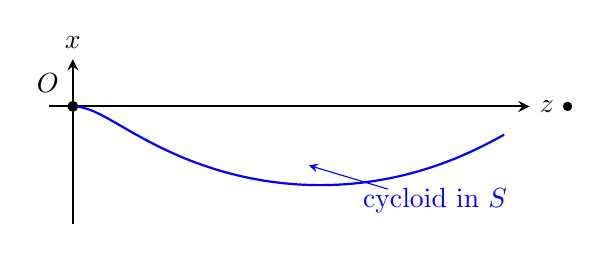
\begin{tikzpicture}[>=stealth, scale=1.0]
  \draw[->, thick] (-0.3,0) -- (5.8,0) node[right] {$z$};
  \draw[->, thick] (0,-1.5) -- (0,0.6) node[above] {$x$};
  \node[circle,fill,inner sep=1.4pt,label=above left:{$O$}] at (0,0) {};
  \draw[thick,blue,domain=0:5.0,smooth,variable=\t,samples=80]
     plot ({\t-0.5*sin(\t r)},{-0.5+0.5*cos(\t r)});
  % cusp markers
  \node[circle,fill,inner sep=1.2pt] at (0,0) {};
  \node[circle,fill,inner sep=1.2pt] at ({2*pi-0.5*sin(2*pi r)},{-0.5+0.5*cos(2*pi r)}) {};
  \node[blue] at (4.6,-1.2) {cycloid in $S$};
  \draw[blue,->,thin] (4.0,-1.05) -- (3.0,-0.75);
\end{tikzpicture}
\end{center}

\boxed{\;|E/B|>c:\text{ accelerated drift; }\;|E/B|<c:\text{ cycloid (}\vb E\times\vb B\text{ drift)}.\;}

\subsection*{(b)}

Use metric $\eta=\diag(-1,+1,+1,+1)$. Faraday tensor components:
\[ F^{0i} = E^i/c,\quad F^{i0} = -E^i/c,\quad F^{ij} = -\epsilon^{ijk}B_k. \]
Use antisymmetry $F^\nu{}_\lambda = -F_\lambda{}^\nu$ to rewrite the first piece in a manifestly cleaner form:
\[ -F^{\mu\lambda}F^\nu{}_\lambda = F^{\mu\lambda}F_\lambda{}^\nu. \]
Lower with $g_{\mu\nu}$: for the mixed time-space component,
\[ F_i{}^0 = g_{ii}\,g^{00}\,F^{i0} = (+1)(-1)(-E^i/c) = +E^i/c. \]
Invariant scalar:
\[ F_{\kappa\lambda}F^{\kappa\lambda} = 2(\vb B^2 - \vb E^2/c^2). \]

\textbf{$T^{00}$.} Contract $F^{0\lambda}F_\lambda{}^0$:
\[ F^{0\lambda}F_\lambda{}^0 = F^{0i}F_i{}^0 = (E^i/c)(E^i/c) = +\vb E^2/c^2. \]
Apply $g^{00}=-1$ to the trace term:
\[ -\tfrac14 g^{00}F_{\kappa\lambda}F^{\kappa\lambda} = -\tfrac14(-1)(2)(\vb B^2-\vb E^2/c^2) = \tfrac12(\vb B^2-\vb E^2/c^2). \]
Substitute into $T^{00} = \epsilon_0 c^2(F^{0\lambda}F_\lambda{}^0 - \tfrac14 g^{00}F_{\kappa\lambda}F^{\kappa\lambda})$:
\[ T^{00} = \epsilon_0 c^2\bigl[\,\vb E^2/c^2 + \tfrac12(\vb B^2-\vb E^2/c^2)\bigr]. \]
Simplify using $c^2 = 1/(\mu_0\epsilon_0)$:
\[ T^{00} = \tfrac12\epsilon_0\vb E^2 + \tfrac{1}{2\mu_0}\vb B^2 \equiv u_{\rm EM}. \]

\textbf{$T^{0i}$.} Since $g^{0i}=0$ the trace term drops:
\[ T^{0i} = \epsilon_0 c^2\, F^{0\lambda}F_\lambda{}^i. \]
For $i=x$, expand the sum over $\lambda$; the $\lambda=0$ piece vanishes since $F^{00}=0$:
\[ F^{0\lambda}F_\lambda{}^x = F^{0y}F_y{}^x + F^{0z}F_z{}^x. \]
Compute $F_j{}^x = g_{jk}g^{xl}F^{kl} = F^{jx}$ in mostly-plus, then $F^{jx} = -\epsilon^{jxk}B_k$:
\[ F_y{}^x = F^{yx} = +B_z,\qquad F_z{}^x = F^{zx} = -B_y. \]
Substitute:
\[ F^{0\lambda}F_\lambda{}^x = (E^y/c)(B_z) + (E^z/c)(-B_y). \]
Recognise the cross product $(\vb E\times\vb B)_x = E^y B^z - E^z B^y$:
\[ F^{0\lambda}F_\lambda{}^x = (\vb E\times\vb B)_x/c. \]
Substitute back:
\[ T^{0x} = \epsilon_0 c^2\cdot (\vb E\times\vb B)_x/c = \epsilon_0 c\,(\vb E\times\vb B)_x. \]
Generalise to all $i$ and use $\epsilon_0 c = 1/(\mu_0 c)$:
\[ T^{0i} = \frac{(\vb E\times\vb B)_i}{\mu_0 c} = \frac{S_i}{c}. \]
Combine:
\begin{equation}
\boxed{\;T^{0\nu} = \left(u_{\rm EM},\;\bm S/c\right) = \left(\tfrac12\epsilon_0\vb E^2 + \tfrac{1}{2\mu_0}\vb B^2,\;\frac{\vb E\times\vb B}{\mu_0 c}\right).\;}
\label{eq:T0nu}
\end{equation}
$T^{00}$ = EM energy density; $T^{0i}$ = $c\times$(momentum density) = energy flux/$c$.

\subsection*{(c)}

\textbf{Plates $\parallel xy$, motion along $\hat{\vb x}$.} Rest frame $S^*$: $\vb E^*=E\hat{\vb z}$, $\vb B^*=0$. Faraday tensor non-zero entries:
\[ F^{*03}=E/c,\qquad F^{*30}=-E/c. \]
Energy density and Poynting:
\[ u^*=\tfrac12\epsilon_0 E^2,\qquad \vb S^*=0. \]
Maxwell stress has tension along $\vb E$ ($\hat{\vb z}$) and pressure transverse ($\hat{\vb x},\hat{\vb y}$); with $(-,+,+,+)$ signature this gives a longitudinal $-u^*$ on the $33$ slot and $+u^*$ on the others:
\[ T^{*\mu\nu}_{(xy)} = u^*\,\diag(+1,+1,+1,-1). \]

Boost to lab along $-\hat{\vb x}$ (capacitor moves at $+v\hat{\vb x}$ relative to lab). Boost matrix:
\[ \Lambda^0{}_0=\gamma,\quad \Lambda^0{}_1=\Lambda^1{}_0=\beta\gamma,\quad \Lambda^1{}_1=\gamma,\quad \Lambda^2{}_2=\Lambda^3{}_3=1. \]
Transform $T^{\mu\nu}\to T'^{\mu\nu} = \Lambda^\mu{}_\alpha\Lambda^\nu{}_\beta T^{*\alpha\beta}$. The $(0,1)$ block of $T^*$ is $\diag(u^*,u^*)$. Compute $T'^{00}$:
\[ T'^{00} = (\Lambda^0{}_0)^2 T^{*00} + (\Lambda^0{}_1)^2 T^{*11} = \gamma^2 u^* + \gamma^2\beta^2 u^*. \]
Factor:
\[ T'^{00} = \gamma^2 u^*(1+\beta^2). \]
Compute $T'^{01}$:
\[ T'^{01} = \Lambda^0{}_0\Lambda^1{}_0 T^{*00} + \Lambda^0{}_1\Lambda^1{}_1 T^{*11} = \gamma\beta\gamma\,u^* + \beta\gamma\,\gamma\,u^*. \]
Simplify:
\[ T'^{01} = 2\gamma^2\beta\, u^*. \]
Compute $T'^{11}$:
\[ T'^{11} = (\Lambda^1{}_0)^2 T^{*00} + (\Lambda^1{}_1)^2 T^{*11} = \gamma^2\beta^2 u^* + \gamma^2 u^*. \]
Simplify:
\[ T'^{11} = \gamma^2 u^*(1+\beta^2). \]
Other components ($T'^{22} = u^*$, $T'^{33} = -u^*$) unchanged. Hence
\begin{equation}
\boxed{\;T^{\mu\nu}_{(xy),\rm lab} = u^*\!\begin{pmatrix}\gamma^2(1+\beta^2)&2\gamma^2\beta&0&0\\ 2\gamma^2\beta&\gamma^2(1+\beta^2)&0&0\\ 0&0&+1&0\\ 0&0&0&-1\end{pmatrix},\;\;u^*=\tfrac12\epsilon_0 E^2.\;}
\end{equation}

\textbf{Plates $\parallel yz$, motion along $\hat{\vb x}$.} Rest frame: $\vb E^*=E\hat{\vb x}$, $\vb B^*=0$. Now $\vb E$ is along $\hat{\vb x}$ so the tension is along the boost direction:
\[ T^{*\mu\nu}_{(yz)} = u^*\,\diag(+1,-1,+1,+1). \]
Boost along $\hat{\vb x}$: $\vb E_\parallel$ unchanged, so $\vb E_{\rm lab} = E\hat{\vb x}$ and $\vb B_{\rm lab}=0$. Equivalently, apply the same $\Lambda$ to $T^*$. Compute $T'^{00}$:
\[ T'^{00} = \gamma^2 T^{*00} + \gamma^2\beta^2 T^{*11} = \gamma^2 u^* - \gamma^2\beta^2 u^* = \gamma^2(1-\beta^2)u^* = u^*. \]
Compute $T'^{01}$:
\[ T'^{01} = \gamma^2\beta(T^{*00} + T^{*11}) = \gamma^2\beta(u^* - u^*) = 0. \]
Compute $T'^{11}$:
\[ T'^{11} = \gamma^2\beta^2 T^{*00} + \gamma^2 T^{*11} = \gamma^2\beta^2 u^* - \gamma^2 u^* = -\gamma^2(1-\beta^2)u^* = -u^*. \]
Stress--energy tensor invariant:
\begin{equation}
\boxed{\;T^{\mu\nu}_{(yz),\rm lab} = u^*\,\diag(+1,-1,+1,+1).\;}
\end{equation}

\textbf{Energy flow.} $T^{0i}$ = energy flux (Poynting / $c$).
\begin{itemize}
\item $(xy)$: $T^{01}=2\gamma^2\beta u^*\neq 0$. Lab sees $\vb B = -\bm v\times\vb E/c^2$ (transverse to motion), so $\vb S=\vb E\times\vb B/\mu_0$ along $+\hat{\vb x}$. Electrostatic energy is convected with the moving capacitor.
\item $(yz)$: $T^{0i}=0$. Field $\parallel$ boost generates no $\vb B$, no $\vb S$. Energy density unchanged in lab; \emph{no} EM energy flux despite the capacitor moving.
\end{itemize}
\boxed{\;\text{Convection only when boost has component }\perp\vb E.\;}

%==================================================================
\section*{Question 4 --- Symmetry, Lorentz group, rotation generators}

\textbf{Problem.} (a) Define symmetry; identify SR's; SR-consistency criterion. (b) Show 2D rotation orthogonal, 1D boost not. (c) $J_3$ generates $R_z(\theta)$; meaning of $[J_i,J_j]$; rotations form a group. (d) Why boosts alone don't form a group; smallest group containing all 3D Lorentz transformations and connection to the rest.

\subsection*{(a)}

A \emph{symmetry} is a transformation of the dynamical variables that leaves the equations of motion form-invariant. By Noether: continuous symmetries $\leftrightarrow$ conservation laws.

\textbf{SR symmetry.} \emph{Lorentz invariance}: laws form-invariant under $\Lambda^\mu{}_\nu$ (boosts $+$ rotations); with translations forms the Poincaré group. Equivalently, $\eta_{\mu\nu}$ and $c$ are invariant.

\textbf{Criterion.} An equation is SR-consistent iff both sides are Lorentz tensors of identical rank/index structure. Example: $\fourv F = m\fourv A$ is consistent (4-vectors); $\bm F=m\bm a$ alone is not (3-vector $\bm F$ does not transform as part of any single 4-vector without $\gamma$).

\subsection*{(b)}

Clockwise 2D rotation:
\[ R(\theta) = \begin{pmatrix}\cos\theta & \sin\theta\\ -\sin\theta & \cos\theta\end{pmatrix}. \]
Transpose:
\[ R^T(\theta) = R(-\theta). \]
Multiply:
\[ R^T R = R(-\theta)R(\theta) = R(0) = I. \]
Hence orthogonal.

1D Lorentz boost (rapidity $\eta$):
\[ \Lambda(\eta) = \begin{pmatrix}\cosh\eta & -\sinh\eta\\ -\sinh\eta & \cosh\eta\end{pmatrix}. \]
Symmetric, so $\Lambda^T=\Lambda$:
\[ \Lambda^T\Lambda = \Lambda^2 = \begin{pmatrix}\cosh 2\eta & -\sinh 2\eta\\ -\sinh 2\eta & \cosh 2\eta\end{pmatrix}\neq I. \]
Boost preserves Minkowski form, not Euclidean: $\Lambda^T\eta\Lambda = \eta$ (pseudo-orthogonal).

\boxed{\;R^TR=I;\;\Lambda^T\Lambda\neq I,\text{ but }\Lambda^T\eta\Lambda=\eta.\;}

\subsection*{(c)}

\textbf{$J_3$ exponentiates.} Compute $J_3^2$ by direct matrix multiplication:
\[ J_3^2 = \begin{pmatrix}0&-i&0\\ i&0&0\\ 0&0&0\end{pmatrix}^2 = \begin{pmatrix}1&0&0\\ 0&1&0\\ 0&0&0\end{pmatrix} \equiv P. \]
Note $P$ is the projector onto the $xy$-plane: $J_3 P = J_3$, $P^2 = P$, so:
\[ J_3^{2k}=P,\qquad J_3^{2k+1}=J_3\quad (k\ge 1). \]
Expand exponential separating even and odd terms:
\[ e^{-i\theta J_3} = I + \sum_{k\ge 1}\frac{(-i\theta)^{2k}}{(2k)!}J_3^{2k} + \sum_{k\ge 0}\frac{(-i\theta)^{2k+1}}{(2k+1)!}J_3^{2k+1}. \]
Substitute the powers:
\[ e^{-i\theta J_3} = I + P\sum_{k\ge 1}\frac{(-\theta^2)^{k}}{(2k)!} + J_3\sum_{k\ge 0}\frac{(-i\theta)^{2k+1}}{(2k+1)!}. \]
Recognise trig series, noting $\sum_{k\ge 1}(-\theta^2)^k/(2k)! = \cos\theta - 1$ and $\sum_{k\ge 0}(-i\theta)^{2k+1}/(2k+1)! = -i\sin\theta$:
\[ e^{-i\theta J_3} = I + P(\cos\theta - 1) - i J_3\sin\theta. \]
Compute $-iJ_3$:
\[ -iJ_3 = \begin{pmatrix}0&-1&0\\ 1&0&0\\ 0&0&0\end{pmatrix}. \]
Assemble matrix:
\[ e^{-i\theta J_3} = \begin{pmatrix}\cos\theta & -\sin\theta & 0\\ \sin\theta & \cos\theta & 0\\ 0 & 0 & 1\end{pmatrix} = R_z(\theta). \]
Hence $J_3$ generates rotation about $\hat{\bm z}$.

\textbf{Lie algebra.}
\[ [J_i,J_j] = i\epsilon_{ijk}J_k. \]
Meaning: structure constants of the rotation group; quantifies non-commutativity of infinitesimal rotations. Two infinitesimal rotations about $\hat{\bm x}$ then $\hat{\bm y}$ differ from the reverse order by a rotation about $\hat{\bm z}$.

\textbf{Group axioms.} Closure: BCH series
\[ e^A e^B = e^{A+B+\tfrac12[A,B]+\dots} \]
involves only nested commutators. By $[J_i,J_j]=i\epsilon_{ijk}J_k$, every commutator stays in $\mathrm{span}\{J_k\}$; so $e^A e^B = e^{-i\theta'\hat n'^k J_k}$, again a rotation. Identity: $R(0)=I$. Inverse: $R(-\theta,\hat{\bm n})$. Associativity: matrix multiplication. All four axioms hold.

\boxed{\;\text{Closure of }[J_i,J_j]\text{ }\Leftrightarrow\text{ rotations form a group SO(3)}.\;}

\subsection*{(d)}

\textbf{Boost commutator:}
\[ [K_i,K_j] = -i\epsilon_{ijk}J_k. \]
Two boosts in different directions yield a \emph{rotation} (Wigner/Thomas) rather than a boost. Hence $\mathrm{span}\{K_i\}$ alone does not close under commutators: not a sub-algebra. By BCH, the product of two non-collinear boosts is a boost composed with a rotation; closure fails.

(Boosts in a fixed direction $\hat{\bm n}$, generated by a single $K_i$, do form a 1-parameter sub-group: rapidities add.)

\textbf{Smallest group.} Add rotations: the full algebra $\{J_i,K_i\}$ obeys
\[ [J_i,J_j]=i\epsilon_{ijk}J_k, \]
\[ [J_i,K_j]=i\epsilon_{ijk}K_k, \]
\[ [K_i,K_j]=-i\epsilon_{ijk}J_k. \]
All commutators close within $\mathrm{span}\{J_i,K_i\}$; exponentiation gives the proper orthochronous Lorentz group:
\boxed{\;\mathrm{SO}^+(1,3).\;}

\textbf{Connection to the wider Lorentz group.} $O(1,3)$ has four disconnected components, classified by $\det\Lambda=\pm 1$ and $\Lambda^0{}_0\gtrless 0$:
\begin{center}
\begin{tabular}{l c c l}
\toprule
component & $\det$ & $\Lambda^0{}_0$ & connector to $\mathrm{SO}^+$\\
\midrule
$\mathrm{SO}^+(1,3)$ & $+1$ & $\ge 1$ & identity\\
$P\cdot\mathrm{SO}^+$ & $-1$ & $\ge 1$ & parity $P:(t,\bm x)\to(t,-\bm x)$\\
$T\cdot\mathrm{SO}^+$ & $-1$ & $\le -1$ & time reversal $T:(t,\bm x)\to(-t,\bm x)$\\
$PT\cdot\mathrm{SO}^+$ & $+1$ & $\le -1$ & $PT$\\
\bottomrule
\end{tabular}
\end{center}
$P,T$ are discrete, not reachable by exponentiating $\{J_i,K_i\}$; appended ``by hand'' to recover full $O(1,3)$.

\end{document}
